\documentclass[a4paper,9pt]{ctexart}
\usepackage{amsmath}
\usepackage{esint}
\usepackage{geometry}
\usepackage{graphicx}
\usepackage{subfig}
\usepackage{float}
\usepackage{tikz}
\usepackage{pgfplots}

\geometry {left=1cm,right=1cm,top=2cm,bottom=2cm}
\pagestyle{empty}
\title{Engineering Thermodynamics Cheatsheet}
\author{anonymous}
\date{2023 fall}
\begin{document}
\maketitle

\section{注意事项}
\noindent
\textbf{可能的限制条件}:简单可压缩系;准静态过程;可逆过程;忽略动位能变化,无其它形式功,绝热;理想气体;比热容为常数;忽略泵功\\
\textbf{作图}:可逆过程用实线,不可逆过程用虚线。\\
“迅速”暗示过程可视为绝热。\\
准静态过程才能用过程方程及相关结论。\\
解答题分析前注意说明以什么为分析对象,以什么为孤立系统。\\
将焓、热关系转换为温度关系时注意强调比热容为定值。\\
功\textbf{一定}要注意区分正负!\\
*下文中热力学循环图中斜直线不代表线性关系,只表示变化趋势。只有水平或竖直直线表示不变量。

\section{基本概念}
\noindent
\textbf{简单可压缩系统}:与外界只有热量及准静态容积变化功(膨胀功或压缩功)交换的可压缩系统。\\
\textbf{准静态过程}:造成系统状态改变的不平衡势差无限小,以致该系统在任意时刻均无限接近平衡态的过程为准静态过程。\\
\textbf{可逆过程}:不存在耗散效应的准静态过程为可逆过程。\\
不能说绝热过程就是等熵过程,必须是可逆绝热过程才是等熵过程。

\section{热力学第一定律}

\subsection{储存能}
\noindent
\textbf{内能}:储存于系统内部的能量。内能是状态参数,可表示为$u=f(T,v)$,其中T是温度,v是比容。\\
\textbf{外部储存能}:包括宏观动能和重力位能。\\
\textbf{系统的总储存能}:总储存能为内能、动能和位能之和,即$E=U+E_k+E_p$。比总能量为$e=u+e_k+e_p=u+\frac{c^2}{2}+gz$

\subsection{闭口系统能量方程}
\noindent
\textbf{热力学第一定律}:设进入系统的热量为$Q$,系统对外做功为$W$,系统内能变化为$\Delta U$,则$Q=\Delta U+W$。这是热力学第一定律的一个基本表达式,称为闭口系统能量方程。\\
\textbf{准静态条件下热力学第一定律的两个解析式}:$\delta q=du+pdv$;$\delta q=dh-vdp$

\subsection{开口系统能量方程}
\noindent
\textbf{开口系统能量方程}:$\delta Q=dE_{c,v}+(h+\frac{c^2}{2}+gz)_{out}\delta m_{out}-(h+\frac{c^2}{2}+gz)_{in}\delta m_{in}+\delta W_{net}$\\
\textbf{轴功}:热力设备与外界交换的机械功,常记为$W_s$。\\
\textbf{技术功}:工程技术上可利用的能量,常记为$W_t$,$W_t=\frac{1}{2}m\Delta c^2+mg\Delta z+W_s$。\\
\textbf{准静态条件下的技术功}:$w_t=-\int vdp$\\
\textbf{膨胀功}:与压缩功同属容积变化功。准静态过程中容积变化功为$W=\int pdV$\\
\textbf{推进功}:又叫流动功,是工质在流动中向前方传递的功,只有在流动时才出现。$w_{in}=p_{in}v_{in}$; $w_{out}=p_{out}v_{out}$\\
\textbf{稳定流动能量方程}:$q=\Delta h+\frac{1}{2}\Delta c^2+g\Delta z+w_{s}$; $q=\Delta h+w_t$\\
\textbf{稳定流动过程中几种功的关系}:$w_{expansion}=\Delta(pv)+w_t$; $w_t=\frac{1}{2}\Delta c^2+g\Delta z+w_s$

\subsection{热力设备}
\noindent
\textbf{稳定流动能量方程}:$q=\Delta h+\frac{1}{2}\Delta c^2+g\Delta z+w_{s}$\\
\textbf{热交换器}:工质流经换热器时,通过管壁与另一种流体交换热量。此时$w_s=0$,$g\Delta z=0$,$\frac{1}{2}\Delta c^2=0$。根据稳定流动能量方程,$q=h_2-h_1$\\
\textbf{动力机械}:利用工质膨胀获得机械功的热力设备,如燃气涡轮、汽轮机等。此时$g\Delta z=0$,$\frac{1}{2}\Delta c^2=0$。工质流经动力机械的过程很短,可视为$q=0$。根据稳定流动能量方程,$w_s=h_1-h_2$。即动力机械对外输出的轴功是靠工质的焓降得来。\\
\textbf{压缩机械}:外界对工质做功以压缩工质的热力设备,如压气机等。此时$g\Delta z=0$,$\frac{1}{2}\Delta c^2=0$。工质流经动力机械的过程很短,可视为$q=0$。根据稳定流动能量方程,$-w_s=h_2-h_1$。即工质在压缩机械中被压缩时外界所做的轴功等于工质的焓增。\\
\textbf{喷管}:令工质压力下降、速度增加的机械。通常,工质位能变化可忽略,即$g\Delta z=0$。由于管内流动,不对外做轴功,$w_s=0$。工质流经动力机械的过程很短,可视为$q=0$。根据稳定流动能量方程,$\frac{1}{2}(c_2^2-c_1^2)=h_1-h_2$。即工质动能增量等于焓降。

\section{理想气体的性质与过程}
\subsection{理想气体状态方程}
\noindent
\textbf{理想气体状态方程}:$pv=RT$; $pV=mRT=nR_mT$\\
$R_m$是摩尔气体常数,又称为通用气体常数,与气体种类无关。$R_m=8.3143\mathrm{J/(mol\cdot K)}$。\\
$R$是气体常数,随气体种类而异。$R$与通用气体常数$R_m$的关系为$R_m=M\cdot R$。对于空气,$R=287.1\mathrm{J/(kg\cdot K)}$。\\
空气摩尔质量:28.9656g/mol。

\subsection{比热容}
\noindent
\textbf{比热容}:系统单位物质温度升高1K所需的热量称为比热容。比定容热容记为$c_V$,比定压热容记为$c_p$。\\
$c_v=\frac{\delta q_v}{dT}$; $c_p=\frac{\delta q_p}{dT}$; 
$c_v=\left(\frac{\partial u}{\partial T}\right)_v$; $c_p=\left(\frac{\partial h}{\partial T}\right)_p$\\
\textbf{比热容关系}:$c_p-c_v=R$(迈耶方程)。比定压热容与比定容热容的比值称为比热比,记为$k$。\\
$k=\frac{c_p}{c_v}$; $c_p=\frac{k}{k-1}R$; $c_v=\frac{1}{k-1}R$\\
\textbf{摩尔热容}:$C_{V,m}=\frac{i}{2}R_m$; $C_{p,m}=\frac{i+2}{2}R_m$。其中$i$为气体分子运动自由度。\\
单原子气体$i=3$,双原子气体$i=5$。适当考虑振动并参照实验数据情况下,多原子气体$i=7$。

\subsection{理想气体的熵}
\noindent
根据$ds=\frac{\delta q_{rev}}{T}$及$\delta q=du+pdv=dh-vdp$,得出$ds=\frac{du}{T}+p\frac{dv}{T}=\frac{dh}{T}-v\frac{dp}{T}$。\\
结合$du=c_vdT$,$dh=c_pdT$,$pv=RT$,得$ds=c_v\frac{dT}{T}+R\frac{dv}{v}=c_p\frac{dT}{T}-R\frac{dp}{p}=c_v\frac{dp}{p}+c_p\frac{dv}{v}$;\\
 $\Delta s=c_v\ln\frac{T_2}{T_1}+R\ln\frac{v_2}{v_1}=c_p\ln\frac{T_2}{T_1}-R\ln\frac{p_2}{p_1}=c_v\ln\frac{p_2}{p_1}+c_p\ln\frac{v_2}{v_1}$


\subsection{绝热过程}
\noindent
绝热过程中$ds=0$,即$c_v\frac{dp}{p}+c_p\frac{dv}{v}=0$,由此得出绝热过程方程:$p\cdot v^k=C$。\\
由过程方程可得出:$\frac{T_2}{T_1}=\left(\frac{v_1}{v_2}\right)^{k-1}$; $\frac{T_2}{T_1}=\left(\frac{p_2}{p_1}\right)^{\frac{k-1}{k}}$。
进一步可推出:\\
\textbf{内能}:$\Delta u=c_v(T_2-T_1)$;\textbf{焓}:$\Delta h=c_p(T_2-T_1)$。\\
\textbf{膨胀功}:$w=-\Delta u=c_v(T_1-T_2)=\frac{R}{k-1}(T_1-T_2)=\frac{1}{k-1}(p_1v_1-p_2v_2)=\frac{1}{k-1}RT_1\left(1-(\frac{p_2}{p_1})^{\frac{k-1}{k}}\right)$\\
\textbf{技术功}:$w_t=-\Delta h=c_p(T_1-T_2)=\frac{kR}{k-1}(T_1-T_2)=\frac{k}{k-1}(p_1v_1-p_2v_2)=\frac{k}{k-1}RT_1\left(1-(\frac{p_2}{p_1})^{\frac{k-1}{k}}\right)$\\
注意到$w_t=kw$,即绝热过程的技术功是膨胀功的$k$倍。

\subsection{多变过程}
\noindent
\textbf{多变过程方程}:$pv^n=C$。其中$n$为多变指数。\\
$n=0$时为定压过程,$n=1$时为定温过程,$n=k$时为等熵过程,$n=\pm\infty$时为定容过程。\\
根据过程方程及状态方程$pv=RT$,可得$\frac{p_2}{p_1}=\left(\frac{v_1}{v_2}\right)^{n}$; $\frac{T_2}{T_1}=\left(\frac{v_1}{v_2}\right)^{n-1}=\left(\frac{p_2}{p_1}\right)^{\frac{n-1}{n}}$\\
\textbf{膨胀功}:$w=\int pdv=\frac{R}{n-1}(T_1-T_2)=\frac{1}{n-1}(p_1v_1-p_2v_2)=\frac{1}{n-1}RT_1\left(1-(\frac{p_2}{p_1})^{\frac{n-1}{n}}\right)$; n=1时,$w=p_1v_1\ln\frac{v_2}{v_1}$\\
\textbf{技术功}:$w_t=-\int vdp=\frac{nR}{n-1}(T_1-T_2)=\frac{n}{n-1}(p_1v_1-p_2v_2)=\frac{n}{n-1}RT_1\left(1-(\frac{p_2}{p_1})^{\frac{n-1}{n}}\right)$; n=1时,$w_t=p_1v_1\ln\frac{v_2}{v_1}$\\
\textbf{热量}:$q=\Delta u+w=c_v(T_2-T_1)+\frac{R}{n-1}(T_1-T_2)=(c_v-\frac{R}{n-1})(T_2-T_1)
=\frac{n-k}{n-1}c_v(T_2-T_1)=c_n(T_2-T_1)$。\\
其中$c_n=\frac{n-k}{n-1}$,称为多变比热容。\\
\textbf{分级压缩中间冷却}:最佳增压比:$\beta=\sqrt[N]{\frac{p_{Z+1}}{p_1}}$


\section{热力学第二定律与熵}
\subsection{热力学第二定律的实质与表述}
\noindent
\textbf{克劳修斯表述}:不可能将热从低温物体传至高温物体而不发生任何变化。\\
\textbf{开尔文表述}:不可能从单一热源取热,使之完全转变为有用功而不引起其他变化。

\subsection{卡诺循环与卡诺定理}
\noindent
\textbf{卡诺循环}:定温吸热,绝热膨胀,定温放热,绝热压缩。\textbf{卡诺循环热效率}:$\eta=1-\frac{T_2}{T_1}$。\\
\textbf{卡诺定理}:在两个不同温度的恒温热源之间工作的所有热机中,以可逆热机的效率为最高。

\subsection{孤立系统熵增原理}
\noindent
\textbf{克劳修斯不等式}:$\oint_{IR}\frac{\delta Q}{T_r}<0$。\textbf{克劳修斯等式}:$\oint_R\frac{\delta Q_{rev}}{T_r}=0$。\\
\textbf{孤立系统做功能力损失}:$\Pi=T_0\Delta S_{iso}$。$T_0$为环境温度。对任何不可逆系统均适用。

\subsection{㶲及其计算}
\noindent
\textbf{热量㶲}:$Q-T_0\int dS$; \textbf{冷量㶲}:$T_0\Delta S-Q$\\
\textbf{稳定流动工质的焓㶲}:$e_x=(h-h_0)-T_0(s-s_0)$(忽略动位能);\textbf{内能㶲}:$e_x=(u-u_0)+p_0(v-v_0)-T_0(s-s_0)$



\section{气体动力循环}

\begin{figure}[H]
\centering
\subfloat%[混合加热循环]
{
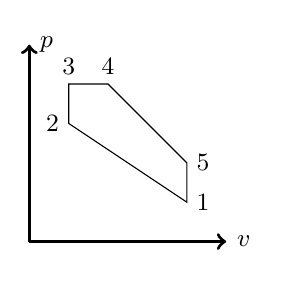
\begin{tikzpicture}[scale=0.5]
\tikzstyle{every node}=[font=\small]
\draw[->,very thick](0,0)--(5,0) node[right]{$v$};
\draw[->,very thick](0,0)--(0,5) node[right]{$p$};
\draw(4,1)node[right]{1}--(1,3)node[left]{2}--(1,4)node[above]{3}--(2,4)node[above]{4}
--(4,2)node[right]{5}--cycle;

\end{tikzpicture}
}
\subfloat%[狄塞尔循环]
{
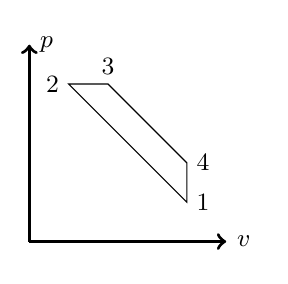
\begin{tikzpicture}[scale=0.5]
\tikzstyle{every node}=[font=\small]
\draw[->,very thick](0,0)--(5,0) node[right]{$v$};
\draw[->,very thick](0,0)--(0,5) node[right]{$p$};
\draw(4,1)node[right]{1}--(1,4)node[left]{2}--(2,4)node[above]{3}--(4,2)node[right]{4}--cycle;
\end{tikzpicture}
}
\subfloat%[奥图循环]
{
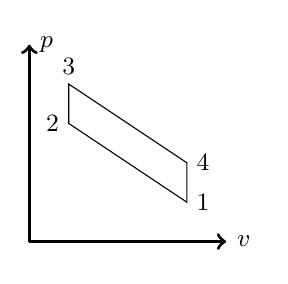
\begin{tikzpicture}[scale=0.5]
\tikzstyle{every node}=[font=\small]
\draw[->,very thick](0,0)--(5,0) node[right]{$v$};
\draw[->,very thick](0,0)--(0,5) node[right]{$p$};
\draw(4,1)node[right]{1}--(1,3)node[left]{2}--(1,4)node[above]{3}--(4,2)node[right]{4}--cycle;
\end{tikzpicture}
}
\subfloat%[斯特林循环]
{
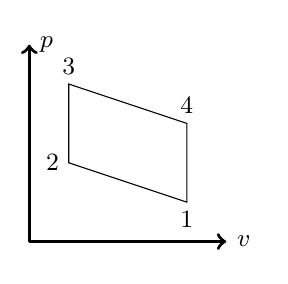
\begin{tikzpicture}[scale=0.5]
\tikzstyle{every node}=[font=\small]
\draw[->,very thick](0,0)--(5,0) node[right]{$v$};
\draw[->,very thick](0,0)--(0,5) node[right]{$p$};
\draw(4,1)node[below]{1}--(1,2)node[left]{2}--(1,4)node[above]{3}--(4,3)node[above]{4}--cycle;
\end{tikzpicture}
}
\quad

\subfloat[混合加热循环]
{
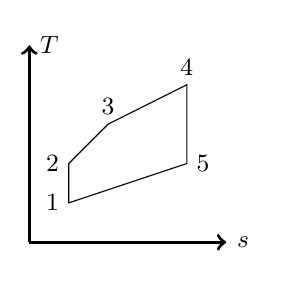
\begin{tikzpicture}[scale=0.5]
\tikzstyle{every node}=[font=\small]
\draw[->,very thick](0,0)--(5,0) node[right]{$s$};
\draw[->,very thick](0,0)--(0,5) node[right]{$T$};
\draw(1,1)node[left]{1}--(1,2)node[left]{2}--(2,3)node[above]{3}--(4,4)node[above]{4}
--(4,2)node[right]{5}--cycle;

\end{tikzpicture}
}
\subfloat[狄塞尔循环]
{
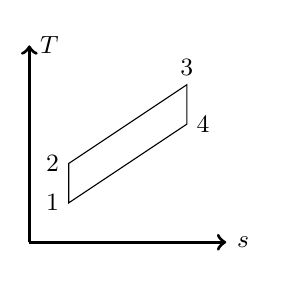
\begin{tikzpicture}[scale=0.5]
\tikzstyle{every node}=[font=\small]
\draw[->,very thick](0,0)--(5,0) node[right]{$s$};
\draw[->,very thick](0,0)--(0,5) node[right]{$T$};
\draw(1,1)node[left]{1}--(1,2)node[left]{2}--(4,4)node[above]{3}--(4,3)node[right]{4}--cycle;
\end{tikzpicture}
}
\subfloat[奥图循环]
{
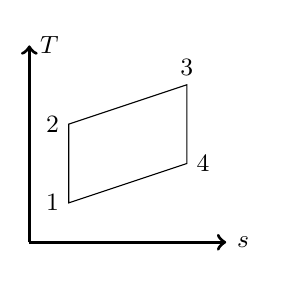
\begin{tikzpicture}[scale=0.5]
\tikzstyle{every node}=[font=\small]
\draw[->,very thick](0,0)--(5,0) node[right]{$s$};
\draw[->,very thick](0,0)--(0,5) node[right]{$T$};
\draw(1,1)node[left]{1}--(1,3)node[left]{2}--(4,4)node[above]{3}--(4,2)node[right]{4}--cycle;
\end{tikzpicture}
}
\subfloat[斯特林循环]
{
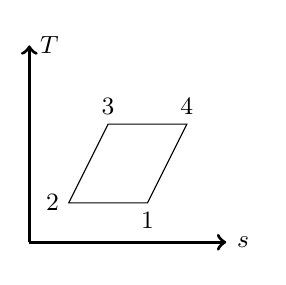
\begin{tikzpicture}[scale=0.5]
\tikzstyle{every node}=[font=\small]
\draw[->,very thick](0,0)--(5,0) node[right]{$s$};
\draw[->,very thick](0,0)--(0,5) node[right]{$T$};
\draw(3,1)node[below]{1}--(1,1)node[left]{2}--(2,3)node[above]{3}--(4,3)node[above]{4}--cycle;
\end{tikzpicture}
}


\end{figure}


\subsection{混合加热循环}
\noindent
\textbf{循环过程}:定熵压缩,定容加热,定压加热,定熵膨胀,定容放热。\\
\textbf{特性参数}:\textbf{压缩比}$\varepsilon=\frac{v_1}{v_2}$,\textbf{定容增压比}$\lambda=\frac{p_3}{p_2}$,\textbf{预胀比}$\rho=\frac{v_4}{v_3}$。\\
\textbf{状态参数关系}:$p_2v_2^k=p_1v_1^k$, $v_3=v_2$, $p_4=p_3$, $p_5v_5^k=p_4v_4^k$\\
\textbf{各点温度}:$T_2=T_1\left(\frac{v_1}{v_2}\right)^{k-1}=T_1\varepsilon^{k-1}$; $T_3=\frac{p_3}{p_2}T_2=\lambda T_2$; $T_4=\frac{v_4}{v_3}T_3=\rho T_3$; $T_5=\frac{p_5}{p_1}T_1$\\
\textbf{吸热量}:$q_{in}=c_v(T_3-T_2)+c_p(T_4-T_3)$;\textbf{放热量}:$q_{out}=c_v(T_5-T_1)$\\
\textbf{热效率}:$\eta_t=1-\frac{\lambda\rho^k-1}{\varepsilon^{k-1}[(\lambda-1)+k\lambda(\rho-1)]}$


\subsection{其它循环}
\noindent
\textbf{定压加热循环(狄塞尔循环)}:定熵压缩,定压加热,定熵膨胀,定容放热。相当于$\lambda=1$,2与3重合。\\
\textbf{定容加热循环(奥图循环)}:定熵压缩,定容加热,定熵膨胀,定容放热。相当于$\rho=1$,3与4重合。\\
\textbf{斯特林循环}:定温压缩,定容吸热,定温膨胀,定容放热。斯特林循环是概括性卡诺循环,$\eta_t=1-\frac{T_L}{T_H}$。\\
斯特林循环不是通过气缸内燃烧取得能量,而是通过气缸外高温热源取得能量,有利于减少污染,利用新能源。

\subsection{勃雷登循环}
\begin{figure}[H]
\centering
\subfloat[勃雷登循环]
{
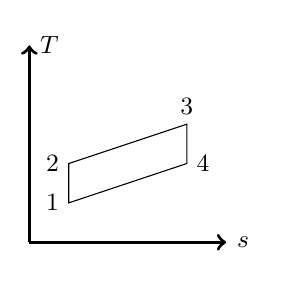
\begin{tikzpicture}[scale=0.5]
\tikzstyle{every node}=[font=\small]
\draw[->,very thick](0,0)--(5,0) node[right]{$s$};
\draw[->,very thick](0,0)--(0,5) node[right]{$T$};
\draw(1,1)node[left]{1}--(1,2)node[left]{2}--(4,3)node[above]{3}--(4,2)node[right]{4}--cycle;
\end{tikzpicture}
}
\subfloat[燃气轮机实际循环]
{
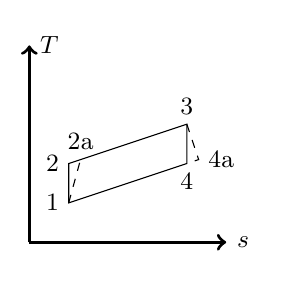
\begin{tikzpicture}[scale=0.5]
\tikzstyle{every node}=[font=\small]
\draw[->,very thick](0,0)--(5,0) node[right]{$s$};
\draw[->,very thick](0,0)--(0,5) node[right]{$T$};
\draw(1,1)node[left]{1}--(1,2)node[left]{2}--(4,3)node[above]{3}--(4,2)node[below]{4}--cycle;
\draw[dashed](1,1)--(1.3,2.1)node[above]{2a};
\draw[dashed](4,3)--(4.3,2.1)node[right]{4a}--(4,2);
\end{tikzpicture}
}
\subfloat[回热勃雷登循环]
{
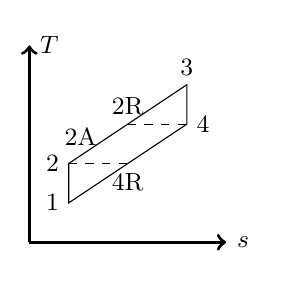
\begin{tikzpicture}[scale=0.5]
\tikzstyle{every node}=[font=\small]
\draw[->,very thick](0,0)--(5,0) node[right]{$s$};
\draw[->,very thick](0,0)--(0,5) node[right]{$T$};
\draw(1,1)node[left]{1}--(1,2)node[left]{2}--(4,4)node[above]{3}--(4,3)node[right]{4}--cycle;
\draw[dashed](1,2)--(2.5,2)node[below]{4R};
\draw[dashed](2.5,3)node[above]{2R}--(4,3);
\draw(1.3,2.2)node[above]{2A};

\end{tikzpicture}
}
\subfloat[分级膨胀中间再热]
{
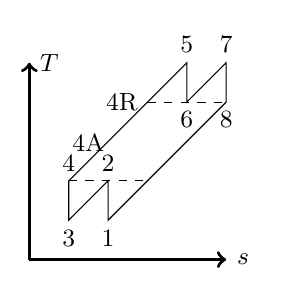
\begin{tikzpicture}[scale=0.5]
\tikzstyle{every node}=[font=\small]
\draw[->,very thick](0,0)--(5,0) node[right]{$s$};
\draw[->,very thick](0,0)--(0,5) node[right]{$T$};
\draw(2,1)node[below]{1}--(2,2)node[above]{2}--(1,1)node[below]{3}--(1,2)node[above]{4}
--(4,5)node[above]{5}--(4,4)node[below]{6}--(5,5)node[above]{7}--(5,4)node[below]{8}--cycle;
\draw[dashed](1,2)--(3,2);
\draw[dashed](3,4)node[left]{4R}--(5,4);
\draw(1.5,2.5)node[above]{4A};
\end{tikzpicture}
}

\end{figure}


\noindent
\textbf{循环过程}:定熵压缩(压气机),定压吸热,定熵膨胀(燃气轮机),定压放热。\\
\textbf{特性参数}:\textbf{循环增压比}$\pi=\frac{p_2}{p_1}$;\textbf{循环增温比}$\tau=\frac{T_3}{T_1}$。\\
\textbf{状态参数关系}:$p_1=p_4$, $p_3=p_2$, $\frac{T_4}{T_3}=\frac{T_1}{T_2}=\left(\frac{p_4}{p_3}\right)^{\frac{k-1}{k}}=\left(\frac{p_1}{p_2}\right)^{\frac{k-1}{k}}$\\
\textbf{热效率}:$\eta_t=1-\frac{q_2}{q_1}=1-\frac{c_p(T_4-T_1)}{c_p(T_3-T_2)}=1-\frac{T_1}{T_2}=1-1/\pi^{\frac{k-1}{k}}$\\
\textbf{压气机做功}:$w_c=\frac{k}{k-1}RT_1\left[1-(\frac{p_2}{p_1})^{\frac{k-1}{k}}\right]$;
\textbf{燃气轮机做功}:$w_T=\frac{k}{k-1}RT_3\left[1-(\frac{p_1}{p_2})^{\frac{k-1}{k}}\right]$\\
\textbf{循环净功}:$w_{net}=(h_3-h_4)-(h_2-h_1)=c_pT_1(\frac{T_3}{T_1}-\frac{T_4}{T_3}\frac{T_3}{T_1}-\frac{T_2}{T_1}+1)=c_pT_1(\tau-\tau\pi^{\frac{1-k}{k}}-\pi^{\frac{k-1}{k}}+1)$。\\
\textbf{最佳增压比}:$\pi_{opt}=\tau^{\frac{k}{2(k-1)}}=\left(\frac{T_3}{T_1}\right)^{\frac{k}{2(k-1)}}$。\textbf{最大循环净功}:$w_{net, max}=c_pT_1(\sqrt{\tau}-1)^2$

\subsection{燃气轮机装置的实际循环}
\noindent
\textbf{压气机绝热效率}:$\eta_c=\frac{h_2-h_1}{h_{2a}-h_1}$;\textbf{燃气轮机相对内效率}:$\eta_{oi}=\frac{h_3-h_{4a}}{h_3-h_4}$。\\
\textbf{实际循环吸热量}:$q_{in}'=h_3-h_{2a}=h_3-h_1-\frac{h_2-h_1}{\eta_c}$\\
\textbf{实际循环净功}:$w_{net}'=(h_3-h_{4a})-(h_{2a}-h_1)=\eta_{oi}(h_3-h_4)-\frac{h_2-h_1}{\eta_c}$
\\
\textbf{实际循环热效率}:$\eta_t'=\frac{w_{net}'}{q_{in}'}=\left(\eta_{oi}(T_3-T_4)-\frac{T_2-T_1}{\eta_{c}}\right)/\left(T_3-T_1-\frac{T_2-T_1}{\eta_c}\right)=\left(\frac{\tau}{\pi^{\frac{k-1}{k}}}\eta_{oi}-\frac{1}{\eta_c}\right)/\left(\frac{\tau-1}{\pi^{\frac{k-1}{k}}-1}-\frac{1}{\eta_c}\right)$
\\
\textbf{最佳增压比}:$\pi_{opt}=(\eta_c\cdot\eta_{oi}\cdot\tau)^{\frac{k}{2(k-1)}}$


\subsection{采用回热的勃雷登循环}
\noindent
\textbf{回热度}:$\sigma=\frac{h_{2A}-h_2}{h_{2R}-h_2}=\frac{T_{2A}-T_2}{T_4-T_2}$。易知$T_{2A}=T_2+\sigma(T_4-T_2)$。\\
\textbf{吸热量}:$q_{in}=h_3-h_{2R}$;\textbf{放热量}:$q_{out}=h_{4R}-h_1$\\
\textbf{条件}:燃气轮机排气温度$T_4$高于压气机出口气温$T_2$。\textbf{好处}:平均吸热温度上升,平均放热温度下降,循环效率提高。
\subsubsection{分级膨胀中间再热}
\noindent
\textbf{压气机耗功}:$w_c=(h_4-h_3)+(h_2-h_1)$;\textbf{燃气轮机做功}:$w_T=(h_5-h_6)+(h_7-h_8)$\\
\textbf{吸热量}:$q_{in}=(h_5-h_{4A})+(h_7-h_6)$;\textbf{循环热效率}:$\eta_t=\frac{w_T-w_c}{q_{in}}$\\
\textbf{状态参数关系}:$\pi=\frac{p_2}{p_1}=\frac{p_4}{p_3}$; $T_4=T_2=T_1\pi^{\frac{k-1}{k}}$; $T_6=T_8=T_5\pi^{-\frac{k-1}{k}}$; $T_{4A}=T_4+\sigma(T_{4R}-T_4)$

\section{水蒸气的性质与过程}
\noindent
\textbf{饱和线}:单相区与两相共存区的分界线称为饱和线。液相区与液-气共存区的分界线称为饱和液体线;气相区与液-气共存区的分界线称为饱和气线;固相区与固-液共存区的分界线称为饱和固体线。水的饱和液体线称为饱和水线(下界线),水的饱和气线称为干饱和气线(上界线),饱和水线和干饱和气线的交界点是水的临界点。
\\
\textbf{临界点}:饱和液体线与饱和气线相交的点称为临界点。临界状态的压力和温度是液相与气相能够平衡共存的最高值。\\
\textbf{三相线}:表征固、液、气相共存。其上的点拥有相同的压力与温度,比容因各物质比例不同而不同。\\
\textbf{饱和状态}:汽化与凝结的分子数处于动态平衡,空间中蒸汽的分子数维持不变。饱和温度与饱和压力一一对应。\\
\textbf{水的五态}:过冷水,饱和水,湿蒸汽,干饱和蒸汽,过热蒸汽。饱和水与过冷水温度之差为过冷度,过热蒸汽与干饱和蒸汽温度之差为过热度。\\
\textbf{状态参数确定原则}:对于简单可压缩工质,只需要两个独立状态参数就可确定出此状态下所有其它参数。饱和水、干饱和蒸汽是单相物质,只需要一个状态参数即可确定其它参数。\\
\textbf{干度}:单位质量湿蒸汽中所含干饱和蒸汽的质量。$x=\frac{m_v}{m_t+m_v}$; $h=xh''+(1-x)h'$; 
$s=xs''+(1-x)s'$; $v=xv''+(1-x)v'$\\
通常规定水三相点的液态水为基准点,以该状态下的液相水的内能和熵为零点。工程上认为该点焓取零也足够准确。\\
\textbf{焓熵图}:定压线群:湿蒸汽区斜率为常数,过热区斜率随温度升高而增大;定温线群:湿蒸汽区定温线与定压线重合,过热蒸汽区变平坦,最终趋于水平;定容线:斜率大于定压线的斜率。\\
\textbf{一点二线三区五态}:一点:临界点;二线:饱和水线(下界线)、干饱和气线(上界线);三区:未饱和水区、湿蒸汽区、过热蒸汽区;五态:过冷水,饱和水,湿蒸汽,干饱和蒸汽,过热蒸汽。


\section{蒸汽动力循环}


%绘制函数:\draw[domain =0:4] plot (\x ,{0.1* exp(\x)}) node[right] {$f(x)=\frac{1}{10}e^x$};
\begin{figure}[H]
\centering
\subfloat[朗肯循环]
{
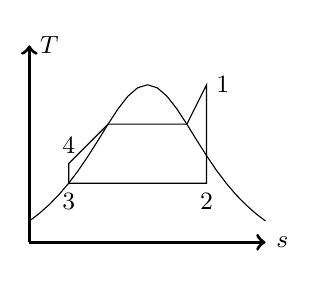
\begin{tikzpicture}[scale=0.5]
\tikzstyle{every node}=[font=\small]
\draw[->,very thick](0,0)--(6,0) node[right]{$s$};
\draw[->,very thick](0,0)--(0,5) node[right]{$T$};
\draw(1,1.5)node[below]{3}--(1,2)node[above]{4}--(2,3)--(4,3)--(4.5,4)node[right]{1}--(4.5,1.5)node[below]{2}--cycle;
\draw[domain =0:6] plot (\x ,{-1+5/(1+(\x-3)^2/4))});

\end{tikzpicture}
}
\subfloat[蒸汽再热循环]
{
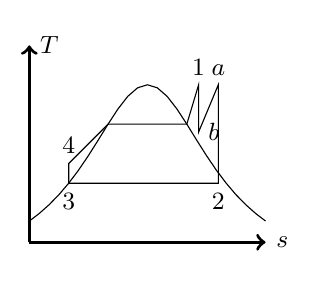
\begin{tikzpicture}[scale=0.5]
\tikzstyle{every node}=[font=\small]
\draw[->,very thick](0,0)--(6,0) node[right]{$s$};
\draw[->,very thick](0,0)--(0,5) node[right]{$T$};
\draw(1,1.5)node[below]{3}--(1,2)node[above]{4}--(2,3)--(4,3)--(4.3,4)node[above]{1}--
(4.3,2.8)node[right]{$b$}--(4.8,4)node[above]{$a$}--(4.8,1.5)node[below]{2}--cycle;
\draw[domain =0:6] plot (\x ,{-1+5/(1+(\x-3)^2/4))});

\end{tikzpicture}
}
\subfloat[蒸汽回热循环]
{
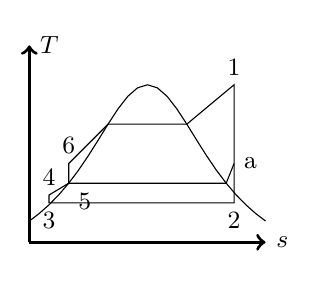
\begin{tikzpicture}[scale=0.5]
\tikzstyle{every node}=[font=\small]
\draw[->,very thick](0,0)--(6,0) node[right]{$s$};
\draw[->,very thick](0,0)--(0,5) node[right]{$T$};
\draw(5.2,4)node[above]{1}--(5.2,2)node[right]{a}--(5.2,1)node[below]{2}--(0.5,1)node[below]{3}--(0.5,1.2)node[above]{4}--(1,1.5)node[below right]{5}--(1,2)node[above]{6}--(2,3)--(4,3)--cycle;
\draw(1,1.5)--(5,1.5)--(5.2,2);



\draw[domain =0:6] plot (\x ,{-1+5/(1+(\x-3)^2/4))});

\end{tikzpicture}
}
\subfloat[空气压缩制冷循环]
{
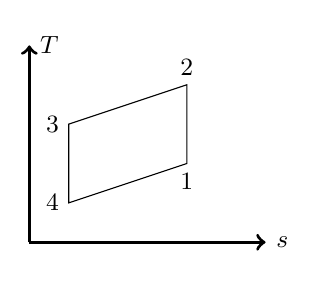
\begin{tikzpicture}[scale=0.5]
\tikzstyle{every node}=[font=\small]
\draw[->,very thick](0,0)--(6,0) node[right]{$s$};
\draw[->,very thick](0,0)--(0,5) node[right]{$T$};
\draw(4,2)node[below]{1}--(4,4)node[above]{2}--(1,3)node[left]{3}--(1,1)node[left]{4}--cycle;

\end{tikzpicture}
}
\subfloat[蒸汽压缩制冷循环]
{
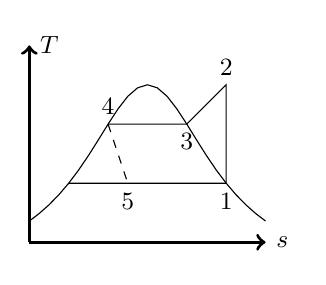
\begin{tikzpicture}[scale=0.5]
\tikzstyle{every node}=[font=\small]
\draw[->,very thick](0,0)--(6,0) node[right]{$s$};
\draw[->,very thick](0,0)--(0,5) node[right]{$T$};
\draw(1,1.5)--(5,1.5)node[below]{1}--(5,4)node[above]{2}--(4,3)node[below]{3}--(2,3)node[above]{4};
\draw[dashed](2,3)--(2.5,1.5)node[below]{5};
\draw[domain =0:6] plot (\x ,{-1+5/(1+(\x-3)^2/4))});

\end{tikzpicture}
}

\end{figure}

\subsection{朗肯循环}
\noindent
\textbf{循环过程}:定熵膨胀(汽轮机),可逆定压放热(冷凝器),定熵压缩(水泵),可逆定压吸热(锅炉)。\\
\textbf{状态参数}:$s_2=s_1$; $h_3=h_2'$; $p_3=p_2$; $s_3=s_2'$; $s_4=s_3$; $p_4=p_1$; \\
汽轮机做功$w_t=h_1-h_2$;水泵耗功$w_p=h_4-h_3\approx v\Delta p$;工质吸热量$q_{in}=h_1-h_4\approx h_1-h_3=h_1-h_2'$\\
\textbf{循环热效率}:$\eta_{t,R}=\frac{(h_1-h_2)-(h_4-h_3)}{h_1-h_4}$。通常忽略泵功,此时$\eta_{t,R}=\frac{h_1-h_2}{h_1-h_3}$\\
\textbf{汽耗率}:蒸汽动力装置输出1kWh功所消耗的蒸汽量。$d=\frac{3600}{w_{net}}$kg/(kWh)\\
为何不采用热效率更高的卡诺循环?因为同温限卡诺循环吸热过程在气态进行,而气态物质实现定温过程非常困难。
\subsection{蒸汽参数对热效率的影响}
\noindent
\textbf{提高初压}:提高热效率;降低出口干度,有危险;降低出口乏汽比容,减小设备尺寸,更经济。\\
\textbf{提高初温}:提高热效率;增大循环功量,降低汽耗率,更经济;增大乏汽干度,更安全;增大乏汽比容,设备尺寸变大,不经济;锅炉过热器和汽轮机高压端要使用昂贵金属材料,不经济。\\
\textbf{降低乏汽压力}:平均吸热温度略降低,平均放热温度明显下降,提高热效率;受环境因素制约。

\subsection{蒸汽再热循环}
\noindent
为避免提高蒸汽初压与初温带来的副作用(见上),常采用蒸汽中间再热。\\
蒸汽在汽轮机中膨胀到某一压力时全部引出,到锅炉再热器中再次加热,然后全部回到汽轮机中继续膨胀做功。\\
\textbf{功}:$w_{RH}=(h_1-h_b)+(h_a-h_2)$;\textbf{循环加热量}:$q_{in,RH}=(h_1-h_4)+(h_a-h_b)$

\subsection{回热循环}
\noindent
新蒸汽在汽轮机中膨胀到一定压力时,抽出$\alpha$kg蒸汽送入回热加热器,其余$(1-\alpha)$kg蒸汽继续膨胀做功到乏汽压力,在冷凝器中冷却成冷凝水,然后经水泵进入回热加热器,被$\alpha$kg的抽汽加热成饱和水,然后经水泵加压,进入锅炉加热、汽化、过热成新蒸汽。\\
\textbf{抽汽率}$\alpha=\frac{h_a'-h_2'}{h_a-h_2'}$;$\alpha h_a+(1-\alpha)h_2'=h_a'$(忽略泵功)\\
\textbf{吸热量}$q_{in}=h_1-h_5=h_1-h_a'=\alpha(h_1-h_a)+(1-\alpha)(h_1-h_2')$;
\textbf{放热量}$q_{out}=(1-\alpha)(h_2-h_2')=(1-\alpha)(h_2-h_3')$\\
\textbf{循环功量}$w=(h_1-h_a)+(1-\alpha)(h_a-h_2)$\\
回热循环热效率大于同参数的朗肯循环效率。由于蒸汽抽出,回热循环的比功小于朗肯循环,汽耗率增大。

\section{制冷及热泵循环}


\subsection{空气压缩制冷循环}
\noindent
\textbf{循环过程}:可逆绝热压缩(压缩机),可逆定压放热(冷却器),可逆绝热膨胀(膨胀机),可逆定压吸热(冷藏室)。\\
\textbf{状态参数}:$\frac{T_2}{T_1}=\left(\frac{p_2}{p_1}\right)^\frac{k-1}{k}=\frac{T_3}{T_4}$\\
吸热量/制冷量$q_{in}=c_p(T_1-T_4)$;放热量$q_{out}=c_p(T_2-T_3)$;
\textbf{制冷系数}$\varepsilon=\frac{q_{in}}{q_{out}-q_{in}}=\frac{T_1}{T_2-T_1}
=1/\left[\left(\frac{p_2}{p_1}\right)^\frac{k-1}{k}-1\right]$\\
\textbf{热泵循环制热系数}:$\varepsilon'=\frac{q_{out}}{w_{net}}=\frac{T_1}{T_1-T_2}$


\subsection{蒸汽压缩制冷循环}
\noindent
\textbf{循环过程}:可逆绝热压缩(压缩机),可逆定压放热(冷凝器),不可逆绝热节流降压降温(节流阀),可逆定压吸热(蒸发器)。
状态1为干饱和蒸汽。4-5为绝热节流过程,不可逆,只能用虚线示意,无确切的中间状态。图中面积不再表示制冷循环的耗功量。\\
吸热量$q_{in}=h_1-h_5=h_1-h_4$;放热量$q_{out}=h_2-h_4$;绝热节流过程性质:$h_4=h_5$;㶲效率:$\eta_{ex}=\varepsilon\left(\frac{T_0}{T_L}-1\right)$\\
$h_1$可由$p_1$确定,$h_2$可由$p_2$和$s_2$确定$(s_2=s_1)$,$h_4$为$p_2$下饱和液体的焓。1冷吨=3.86kW。\\
蒸汽压缩制冷循环的制冷系数低于同温限卡诺循环,但与空气压缩制冷循环相比,它减小了吸热、放热中的温差传热不可逆性,增加了单位质量的制冷量,因为这时吸热过程是依靠工质的气化吸热而非升温吸热,而通常气化潜热较大。

\subsection{制冷剂}
\noindent
\textbf{对制冷剂的热力学要求}:标准大气压下饱和温度(沸点)要低,一般低于-10摄氏度;蒸发温度对应的饱和压力不应过低,最好稍高于大气压力,防止空气漏入系统;冷凝温度对应的饱和压力不宜过高,降低设备耐压密封要求;工作温度范围内汽化潜热要大,以便单位工质有较大制冷能力;临界温度应远高于环境温度,使循环不在临界点附近运行,而运行在具有较大气化潜热的范围之内;凝固点要低,避免低温下凝固阻塞管路;饱和气比容要小,减小设备体积。此外,还要求传热性能良好,溶油性好,化学性质稳定,无腐蚀作用,不可燃,无毒,泄露易被检测,价廉,环保等。


\section{热力学微分关系式及实际气体的性质}
\noindent
\textbf{亥姆霍兹函数}:$f=u-Ts$; $df=du-Tds-sdT=-sdT-pdV$。代表可逆定温条件下内能可以自由转变为功的那部分。\\
\textbf{吉布斯函数}:$g=h-Ts$; $dg=dh-Tds-sdT=-sdT+vdp$。代表可逆定温条件下焓可以自由转变为功的那部分。\\
\textbf{吉布斯方程}:$du=Tds-pdv$; $dh=Tds+vdp$; $df=-sdT-pdv$; $dg=-sdT+vdp$\\
\textbf{全微分条件}:当$z=z(x,y)$,有$dz=Mdx+Ndy$,此时应有$\left(\frac{\partial M}{\partial y}\right)_x=\left(\frac{\partial N}{\partial x}\right)_y$,即$\frac{\partial^2z}{\partial x\partial y}=\frac{\partial^2z}{\partial y\partial x}$\\
\textbf{循环关系式}:$\left(\frac{\partial x}{\partial y}\right)_z\left(\frac{\partial y}{\partial z}\right)_x\left(\frac{\partial z}{\partial x}\right)_y=-1$\ \
\textbf{倒数式}:$\left(\frac{\partial x}{\partial y}\right)_z\left(\frac{\partial y}{\partial x}\right)_z=1$\\
\textbf{链式}:$\left(\frac{\partial x}{\partial y}\right)_w\left(\frac{\partial y}{\partial z}\right)_w\left(\frac{\partial z}{\partial x}\right)_w=1$\ \
\textbf{不同下标式}:$\left(\frac{\partial x}{\partial w}\right)_z=\left(\frac{\partial x}{\partial w}\right)_y+\left(\frac{\partial x}{\partial y}\right)_w\left(\frac{\partial y}{\partial w}\right)_z$\\
\textbf{麦克斯韦关系}:
$\left(\frac{\partial T}{\partial v}\right)_s=-\left(\frac{\partial p}{\partial s}\right)_v$; 
$\left(\frac{\partial T}{\partial p}\right)_s=\left(\frac{\partial v}{\partial s}\right)_p$; 
$\left(\frac{\partial v}{\partial T}\right)_p=-\left(\frac{\partial s}{\partial p}\right)_T$; 
$\left(\frac{\partial p}{\partial T}\right)_v=\left(\frac{\partial s}{\partial v}\right)_T$\\
\textbf{偏导数关系}:
$\left(\frac{\partial u}{\partial s}\right)_v=T$; 
$\left(\frac{\partial u}{\partial v}\right)_s=-p$; 
$\left(\frac{\partial h}{\partial s}\right)_p=T$; 
$\left(\frac{\partial h}{\partial p}\right)_s=v$; 
$\left(\frac{\partial f}{\partial v}\right)_T=-p$; 
$\left(\frac{\partial f}{\partial T}\right)_v=-s$; 
$\left(\frac{\partial g}{\partial p}\right)_T=v$; 
$\left(\frac{\partial g}{\partial T}\right)_p=-s$\\
\textbf{弹性系数}$\alpha_v=\frac{1}{p}\left(\frac{\partial p}{\partial T}\right)_v$;
\textbf{定压热膨胀系数}$\alpha_p=\frac{1}{v}\left(\frac{\partial v}{\partial T}\right)_p$;
\textbf{定温压缩系数}$\beta_T=-\frac{1}{v}\left(\frac{\partial v}{\partial p}\right)_T$;
\textbf{绝热压缩系数}$\beta_s=-\frac{1}{v}\left(\frac{\partial v}{\partial p}\right)_s$\\
\textbf{热系数关系:}$\alpha_p=\alpha_v\cdot\beta_T\cdot p$\\
%\left(\frac{\partial }{\partial }\right)_
\textbf{第一ds方程}:$ds=\frac{c_v}{T}dT+\left(\frac{\partial p}{\partial T}\right)_vdv$\\
\textbf{第二ds方程}:$ds=\frac{c_p}{T}dT-\left(\frac{\partial v}{\partial T}\right)_pdp$\\
\textbf{第三ds方程}:$ds=\left[\frac{c_p}{T}\left(\frac{\partial T}{\partial p}\right)_v-\left(\frac{\partial v}{\partial T}\right)_p\right]dp+\frac{c_p}{T}\left(\frac{\partial T}{\partial v}\right)_pdv$\\
\textbf{第一du方程}:$du=c_vdT+\left[T\left(\frac{\partial p}{\partial T}\right)_v-p\right]dv$\\
\textbf{第二du方程}:$du=\left[c_p-p\left(\frac{\partial v}{\partial T}\right)_p\right]dT-\left[
T\left(\frac{\partial v}{\partial T}\right)_p+p\left(\frac{\partial v}{\partial p}\right)_T\right]dp$\\
\textbf{第三du方程}:$du=\left[c_p\left(\frac{\partial T}{\partial p}\right)_v-T\left(\frac{\partial v}{\partial T}\right)_p\right]dp+\left[c_p\left(\frac{\partial T}{\partial v}\right)_p-p\right]dv$\\
\textbf{第一dh方程}:$dh=\left[c_v+v\left(\frac{\partial p}{\partial T}\right)_v\right]dT+\left[
T\left(\frac{\partial p}{\partial T}\right)_v+v\left(\frac{\partial p}{\partial v}\right)_T\right]dv$\\
\textbf{第二dh方程}:$dh=c_pdT+\left[v-T\left(\frac{\partial v}{\partial T}\right)_p\right]dp$\\
\textbf{第三dh方程}:$dh=c_p\left(\frac{\partial T}{\partial v}\right)_pdv+\left[c_p\left(\frac{\partial T}{\partial p}\right)_v-T\left(\frac{\partial v}{\partial T}\right)_p
+v\right]dp$\\
\textbf{比热容与压力和比容的关系}:$\left(\frac{\partial c_v}{\partial v}\right)_T=T\left(\frac{\partial^2p}{\partial T^2}\right)_v$; $\left(\frac{\partial c_p}{\partial p}\right)_T=-T\left(\frac{\partial^2v}{\partial T^2}\right)_p$\\
\textbf{$c_p$与$c_v$的关系}:$c_p-c_v=T\left(\frac{\partial p}{\partial T}\right)_v\cdot\left(\frac{\partial v}{\partial T}\right)_p=-T\left(\frac{\partial v}{\partial T}\right)_p^2\cdot\left(\frac{\partial p}{\partial v}\right)_T$\\
\textbf{克拉贝龙方程}:$\left(\frac{dp}{dT}\right)_s=\frac{h''-h'}{T_s(v''-v')}=\frac{r}{T_s(v''-v')}$。$r$表示气化潜热。它提供了一种由测得的$p,v,T$计算相变焓变$h''-h'$的途径。
\textbf{焦-汤系数}:$\mu_J=\left(\frac{\partial T}{\partial p}\right)_h$。用于度量绝热节流过程中流体温度变化。其它表示:$\mu_J=-\left(\frac{\partial h}{\partial p}\right)_T/c_p$; 
$\mu_Jc_p=T\left(\frac{\partial v}{\partial T}\right)_p-v$\\
正的焦-汤系数表示绝热节流降压后流体温度将随之降低,负的焦-汤系数象征温度将提高。理想气体的焦-汤系数为零。\\
\textbf{压缩因子}:$Z=\frac{pv}{RT}$。理想气体$Z=1$,实际气体的$Z$或大于1或小于1。\\
\textbf{维里方程}:$Z=1+B'p+C'p^2+\cdots$; $Z=1+\frac{B}{v}+\frac{C}{v^2}+\cdots$。\\
\textbf{范德瓦尔状态方程}:$\left(p+\frac{a}{v^2}\right)(v-b)=RT$; $p=\frac{RT}{v-b}-\frac{a}{v^2}$


\section{化学热力学基础}
\noindent
\textbf{热力学第一定律}:$Q=U_P-U_R+W$。通常只考虑简单可压缩系统,不涉及电磁功等其他形式功,$W$为容积变化功,对外做功为正。\\
\textbf{化学反应热效应}:1kmol主要反应物或生成物所吸收或放出的热量称为反应热效应,规定吸热时热效应为正。定压热效应记作$Q_p$,定容热效应记作$Q_v$。统一规定101.325kPa,25摄氏度为热化学的标准状态,此时的定压热效应为标准定压热效应,记作$Q_p^\circ$。\\
\textbf{燃烧热值}:1kmol燃料完全燃烧时热效应的相反值。\\
\textbf{标准生成焓}:规定任何单质在101.325kPa,25摄氏度条件下焓值为0,有关单质在该条件下通过化学反应生成1kmol化合物所吸收的热量称为该化合物的标准生成焓,用$\bar{h}^\circ_f$表示。\\
\textbf{理想气体反应热效应关系}:$Q_p-Q_v=(n_P-n_R)R_mT$。其中$n_R$和$n_P$分别为反应物和生成物的总摩尔数。\\
\textbf{化学反应中的最大有用功}:稳定流动系统进行可逆定温反应时,系统对外做的最大有用功等于系统吉布斯函数的减少。\\$W_{max}=\sum_Rn_{in}G_{in}-\sum_Pn_{out}G_{out}$。\\
\textbf{物理㶲}:系统经过可逆物理过程达到与环境的温度、压力相平衡的状态(物理死态)所能提供的最大有用功。\\
\textbf{化学㶲}:系统与环境之间由物理死态经可逆物理(扩散)或化学(反应)过程达到与环境化学平衡时能提供的最大有用功。\\
\textbf{㶲损失}:$\Pi=T_0\Delta S_{iso}$。
$\Delta S_{iso}=\left(\sum_Pn_{out}S_{m,out}-\sum_Rn_{in}S_{m,in}\right)+\left(-\frac{Q}{T_0}\right)$\\
$T_0$为环境的热力学温度,$\Delta S_{iso}$为反应系统与环境组成的孤立系统的熵增,$Q$为开口系统向外放出的热量,本身为负值。\\
\textbf{一般情况下反应物的熵}:$S_m(T,p_i)=S_m(T,p_0)-R_m\ln\frac{p_i}{p_0}$\\
\textbf{孤立系统平衡的熵判据}:$dS=0$. $d^2S<0$。\\
\textbf{定温定容反应系统的亥姆霍兹函数判据}:$dF=0$. $d^2F>0$。\\
\textbf{定温定压反应系统的吉布斯函数判据}:$dG=0$. $d^2G>0$。\\
\textbf{反应度}:$\varepsilon=\frac{n_{max}-n}{n_{max}-n{min}}$。\textbf{离解度}:
$\alpha=1-\varepsilon$。\\
\textbf{吉布斯函数}:对于1kmol理想气体,$G_m=G_m^\circ+R_mT\ln\left(\frac{p}{p_0}\right)$。$G_m$是理想气体在$(T,p)$状态下的千摩尔吉布斯函数;$G_m^\circ$是该气体在$(T,101.325\mathrm{K})$状态下的千摩尔吉布斯函数,只与温度有关。$p_0$为标准压力101.325kPa。\\
\textbf{化学反应等温方程式}:$dG_{T,p}=R_mT\left[-\ln K_p+\ln\frac{p_C^cp_D^d}{p_A^ap_B^b}(p_0)^{(a+b-c-d)}\right]d\varepsilon$。可用于判断化学反应的方向以及是否平衡。\\
\textbf{化学平衡常数}:$\ln K_p=-\frac{\Delta G^\circ}{R_mT}$;$K_p=\frac{p_C^cp_D^d}{p_A^ap_B^b}(p_0)^{(a+b-c-d)}$\\
\textbf{范特霍夫方程}:$\frac{d\ln K_p}{dT}=\frac{\Delta H^\circ(T)}{R_mT^2}$。可用于证明温度变化对吸热、放热反应的化学平衡的影响。\\
\textbf{平衡移动原理}:把平衡态的某一因素加以改变后,将使平衡态向着削弱该因素影响的方向转移。\\
\textbf{热力学第三定律}:开尔文温度趋近于0度时,凝聚系统经过任何可逆等温过程,熵的变化趋近于0,即$lim_{T\to 0}(\Delta S)_T=0$;不可能靠有限的步骤使物体的温度达到绝对零度。\\
\textbf{绝对熵}:$S=\int_0^Tc_v\frac{dT}{T}$。



\end{document}